\section{Data Preparation}

\subsection{What was your data source (e.g., web scraping, corporate data, a standard machine learning data set, open data, etc.)?}

Lorem ipsum dolor sit amet, consectetur adipisicing elit. Architecto at aut beatae commodi consequatur eaque fugit, harum hic impedit in incidunt inventore odio officia ratione tenetur totam veritatis. Debitis, magnam.

\subsection{How good was the data quality?}

Lorem ipsum dolor sit amet, consectetur adipisicing elit. Architecto at aut beatae commodi consequatur eaque fugit, harum hic impedit in incidunt inventore odio officia ratione tenetur totam veritatis. Debitis, magnam.

\subsection{What did you need to do to procure it?}

Lorem ipsum dolor sit amet, consectetur adipisicing elit. Architecto at aut beatae commodi consequatur eaque fugit, harum hic impedit in incidunt inventore odio officia ratione tenetur totam veritatis. Debitis, magnam.

\subsection{What tools or code did you need to use to prepare it for analysis?}

For chickens, the raw had to be transformed... etc. Talk about NL data being excluded and the provincial data being aggregated by annual mean; see Figure \ref{fig:chicken_prices}

Please refer to Figure \ref{fig:chicken_production}

\subsection{What challenges did you face?}

Lorem ipsum dolor sit amet, consectetur adipisicing elit. Architecto at aut beatae commodi consequatur eaque fugit, harum hic impedit in incidunt inventore odio officia ratione tenetur totam veritatis. Debitis, magnam.



\begin{figure}
    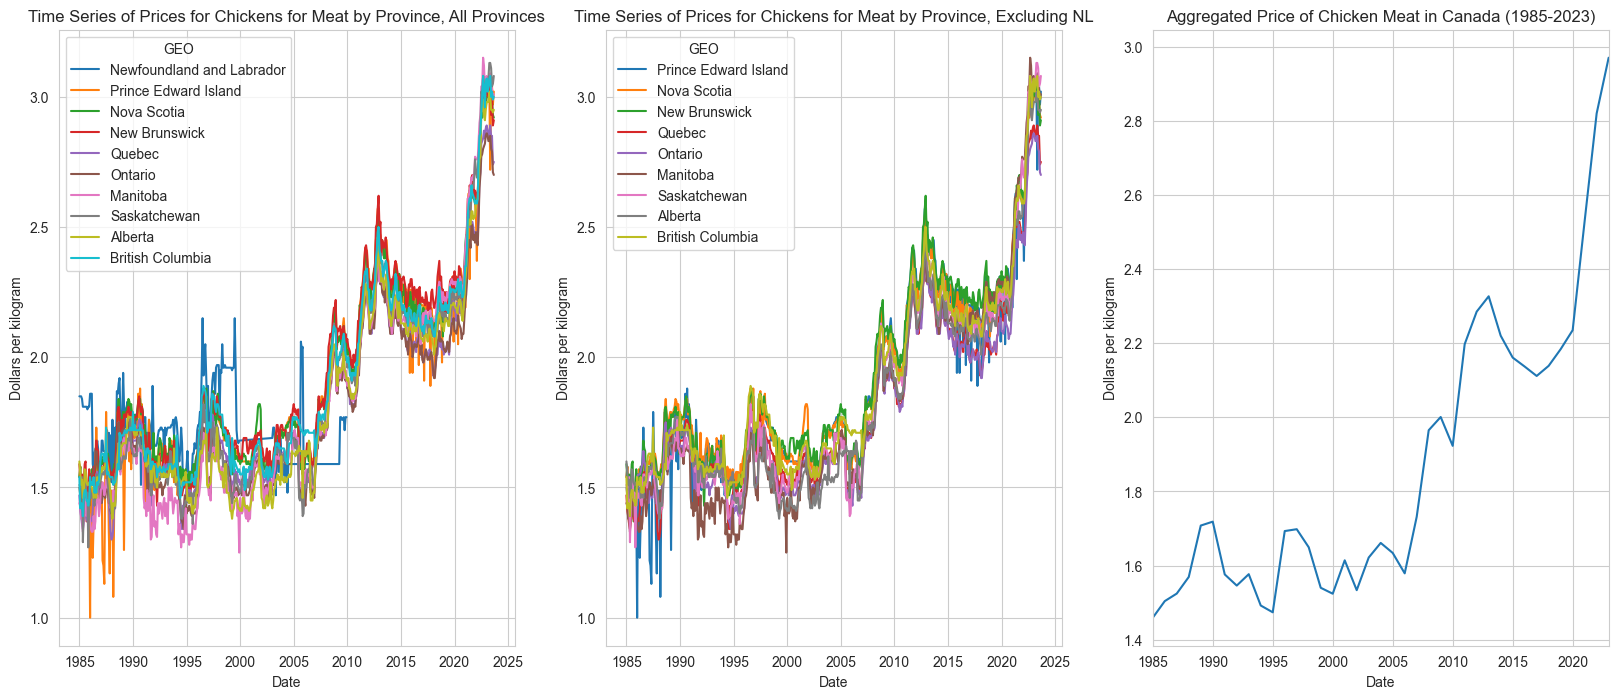
\includegraphics[width=\linewidth]{chicken_prices}
    \caption{This figure shows the raw data, and aggregated forms of chicken prices. MORE TEXT NEEDED?}
    \label{fig:chicken_prices}
\end{figure}


\begin{figure}
    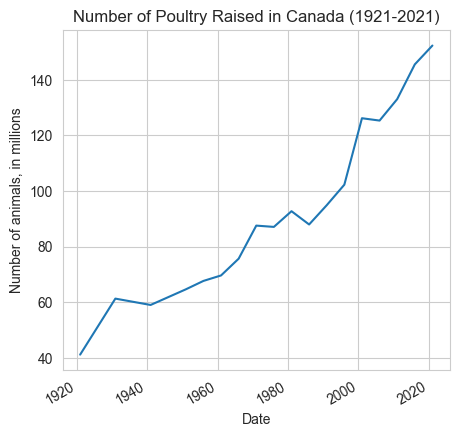
\includegraphics[width=\linewidth]{chicken_production_time_series}
    \caption{This figure shows the number of chickens counted on chicken farms in Canada between 1921-2021.}
    \label{fig:chicken_production}
\end{figure}